\section{Planning phase}
	In this section it will be described how the project startet
	and how the project was defined with scope and requirements.

\subsection{Getting to know each other and the customer}
	At the kickoff of the project, the groups and the customer did not know 
	each other. The fist thing the course staff did was to set all the groups
	together and introduce them to the customer. 

	After the introduction to the course, the students sat down and talked while
	all the customers had a lunch. Later that they, all the groups had a meeting 
	with the customer. At this meeting, the group and the students, sat down and 
	the customer talked about their company. When the students knew some more about
	the customer, the project and the requirements was in focus. 

	In the end of the meeting, the customer wanted the students to come up
	with a game concept and a requirement specification. 
	

\subsection{Project Assignment}
	Before the project started the group got a description of the problem
	in the compendium that was handed out to the course memembers. The 
	description from Helgelandskraft was: 
		\paragraph{Power Control Game}
		{\it The idea is to make a casual game for mobile devices focused around controlling 
		power production from hydro plants trough a power grid to large industry customers and 
		regular consumers, or some other casual game involving power grids, hydro plants 
		and/or other themes around hydro power. 
		 
		The application should also provide the user with power preservation tips, like a 
		tip on loading screens or the splash screen when opening the game. Tips like: 
		 
		“19-21 degrees celsius is a good inside temperature. For each degree you lower the temperature 
		you’ll save 5 procent of the energy used for heating up your living space. 
		You can lower the temperature even more in rooms you normally don’t use.” 
		 
		The application should be developed for iOS and Android. We’ll provide the 
		students with the required equipment needed for iOS-development if they don’t 
		have it, and an android phone if they need it. 
		 
		The application should be designed for the tips and the language to easily be changed.}

	Helgelandskraft wanted a game running on android and Ios, with main theme "power".
	In the project description they introduced some key points, but they did not have a
	concrete idea of what they realy wanted. The scoping of the project and the developing
	of the game project was the next phase to do.

\subsection{Define the Project Scope}


\subsection{Preliminary studies and Project Planning}
	Before starting the project, we needed to do some reseach on project methodology, 
	game concepts and technology. This was a important phase since this type of 
	project was new to the students. 

	\begin{figure}[H]
		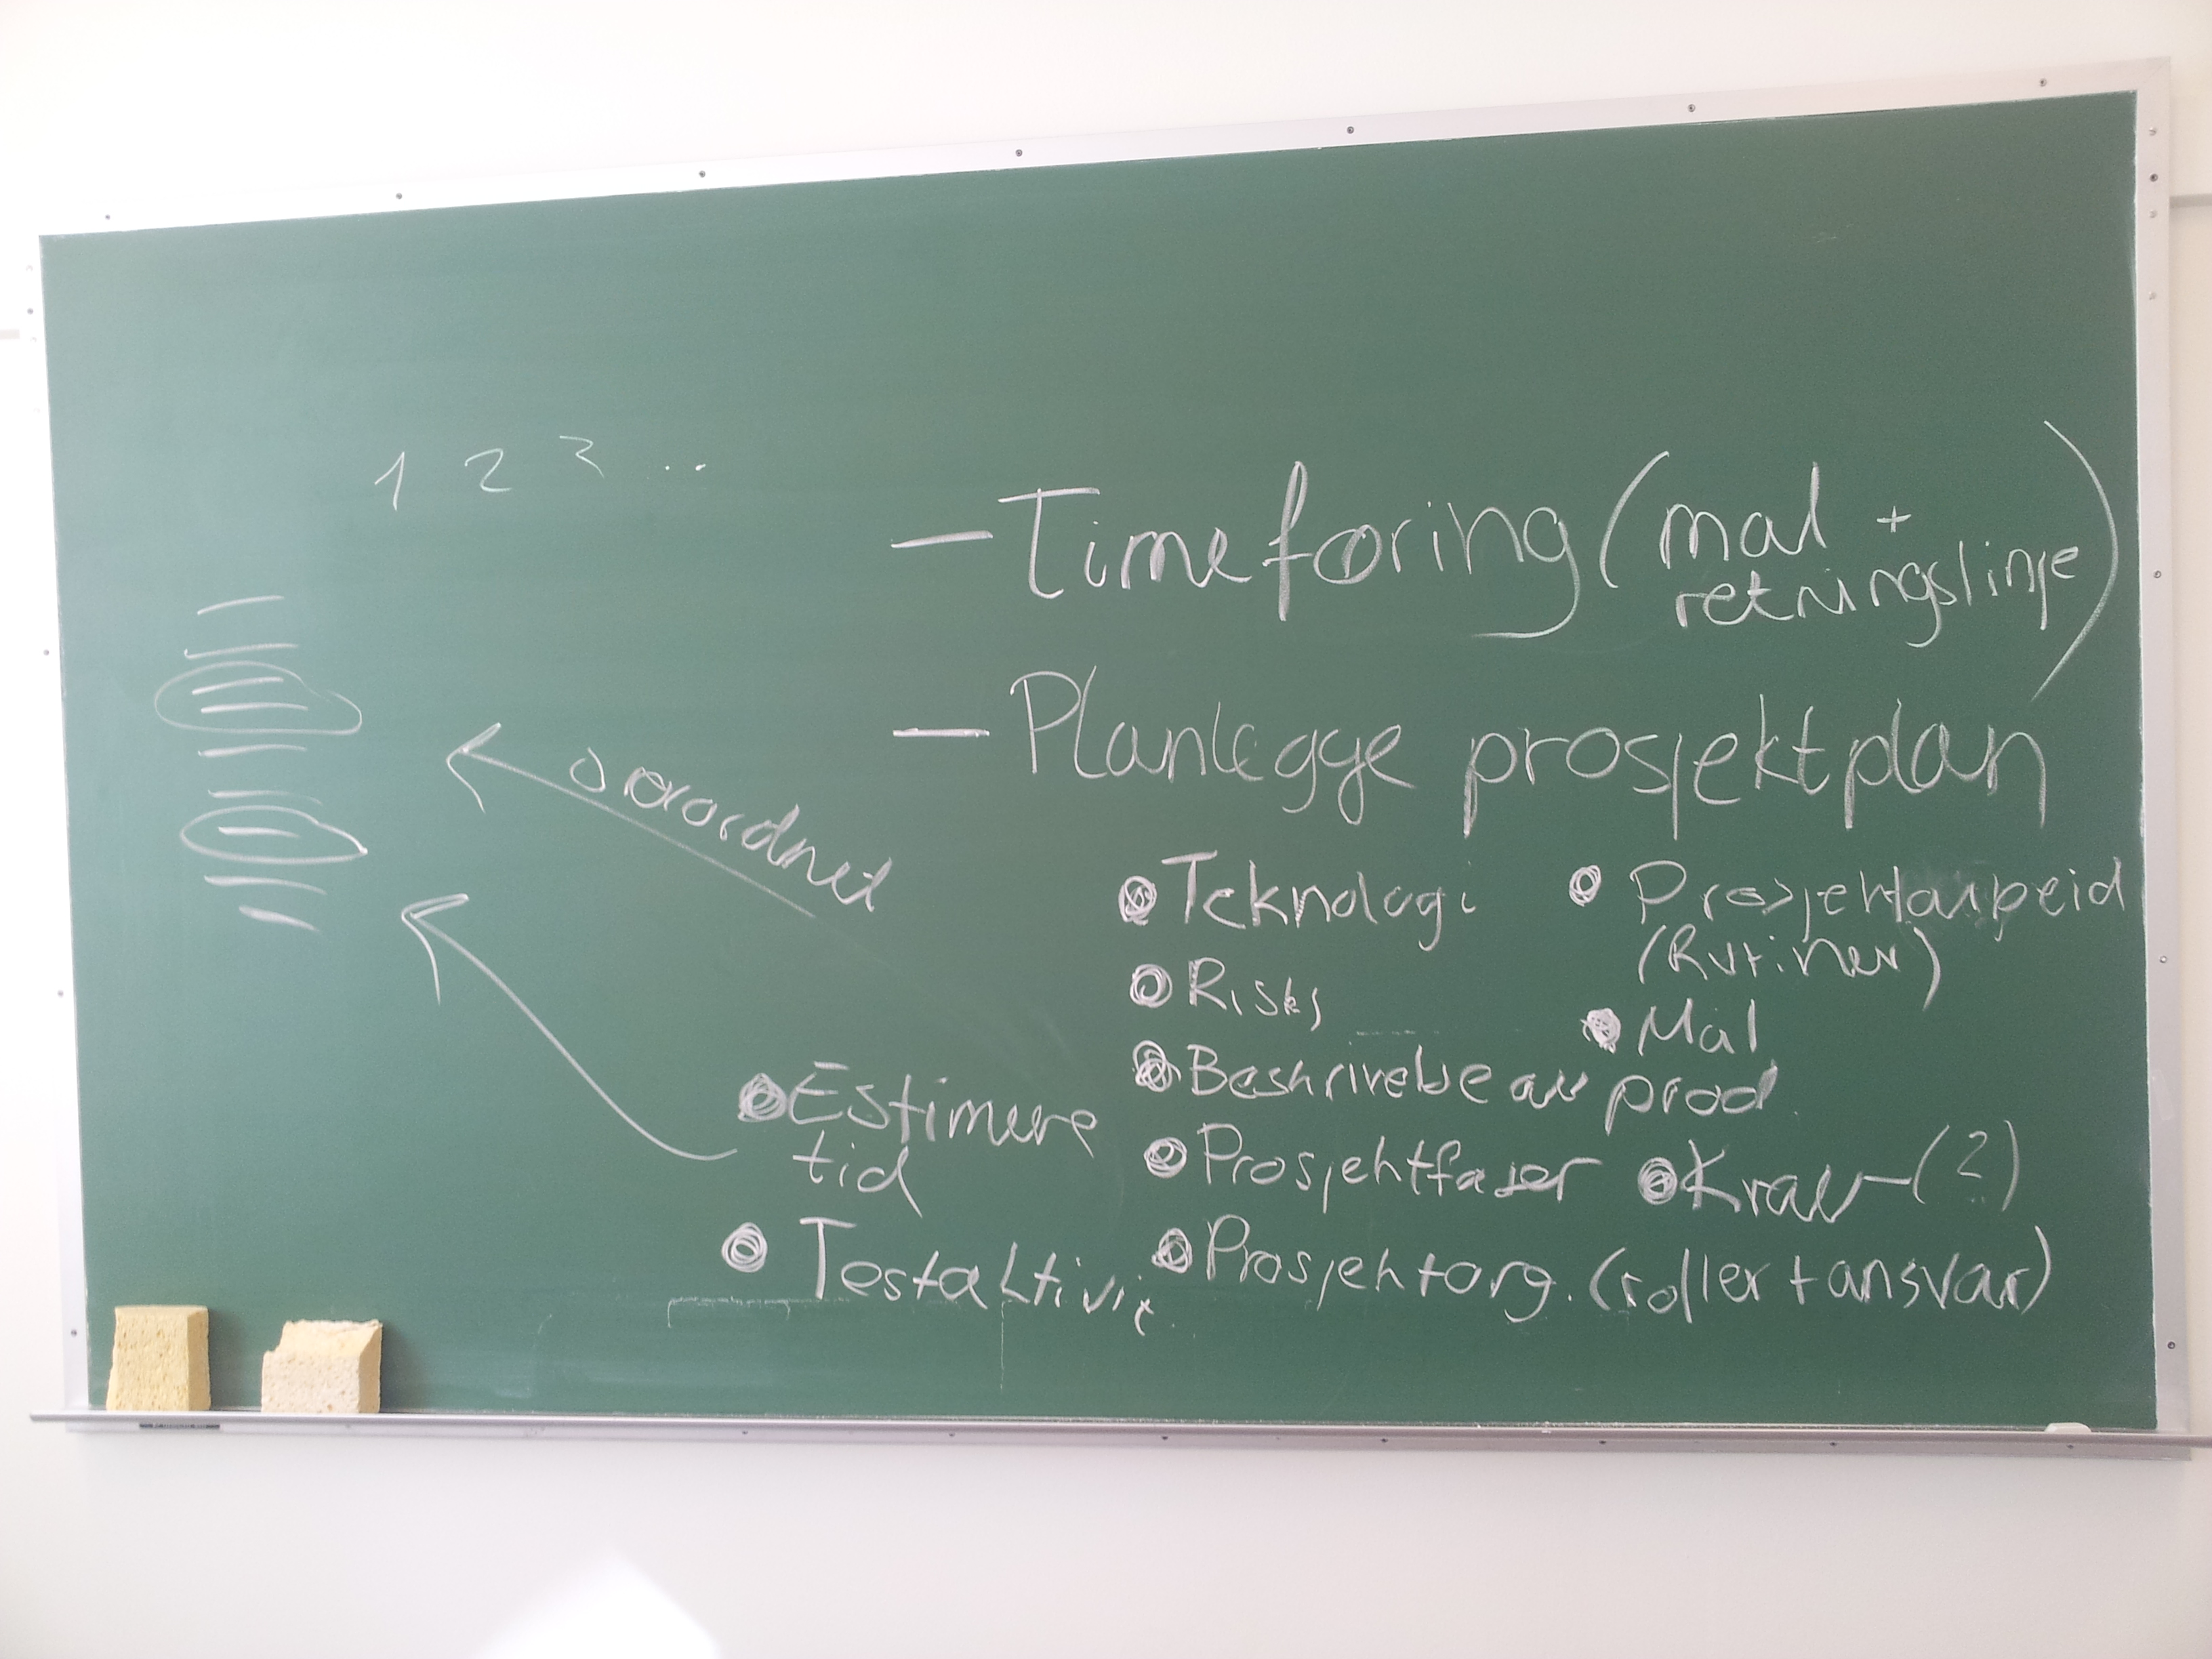
\includegraphics[scale=0.10]{pictures/projectPlanning.jpg}
	\end{figure}

\subsection{Game Concept Development}
	The customer did not know what they wanted the students to deliver in the end of 
	this project. The only thing they knew was that they wanted a power-game that
	was running on android and Ios. 

	The group sat down in a "green zone". The green zone consept is that each team member
	is sitting 10 minutes alone and try to coming up with a concept. After the 10 minutes
	all the members presents their ideas to the rest of the team members.
	After presenting all the consepts, the grpup picked out the best ideas. 

	The first concept was a "shortest-path-problem" game where the player should
	connect a number of nodes with lines without crossing the lines. The goal 
	wad to get the shortest path between the nodes. When the group presented this
	to the customer, they liked the idea, but they wanted a more "real life" game.

	The next concept was a "sim city" like concept, and is the game concept that
	we chose do implement. A description of this can you find in the "Game Concept"
	section. 

	\begin{figure}[H]
	\centering
		\subfigure{
			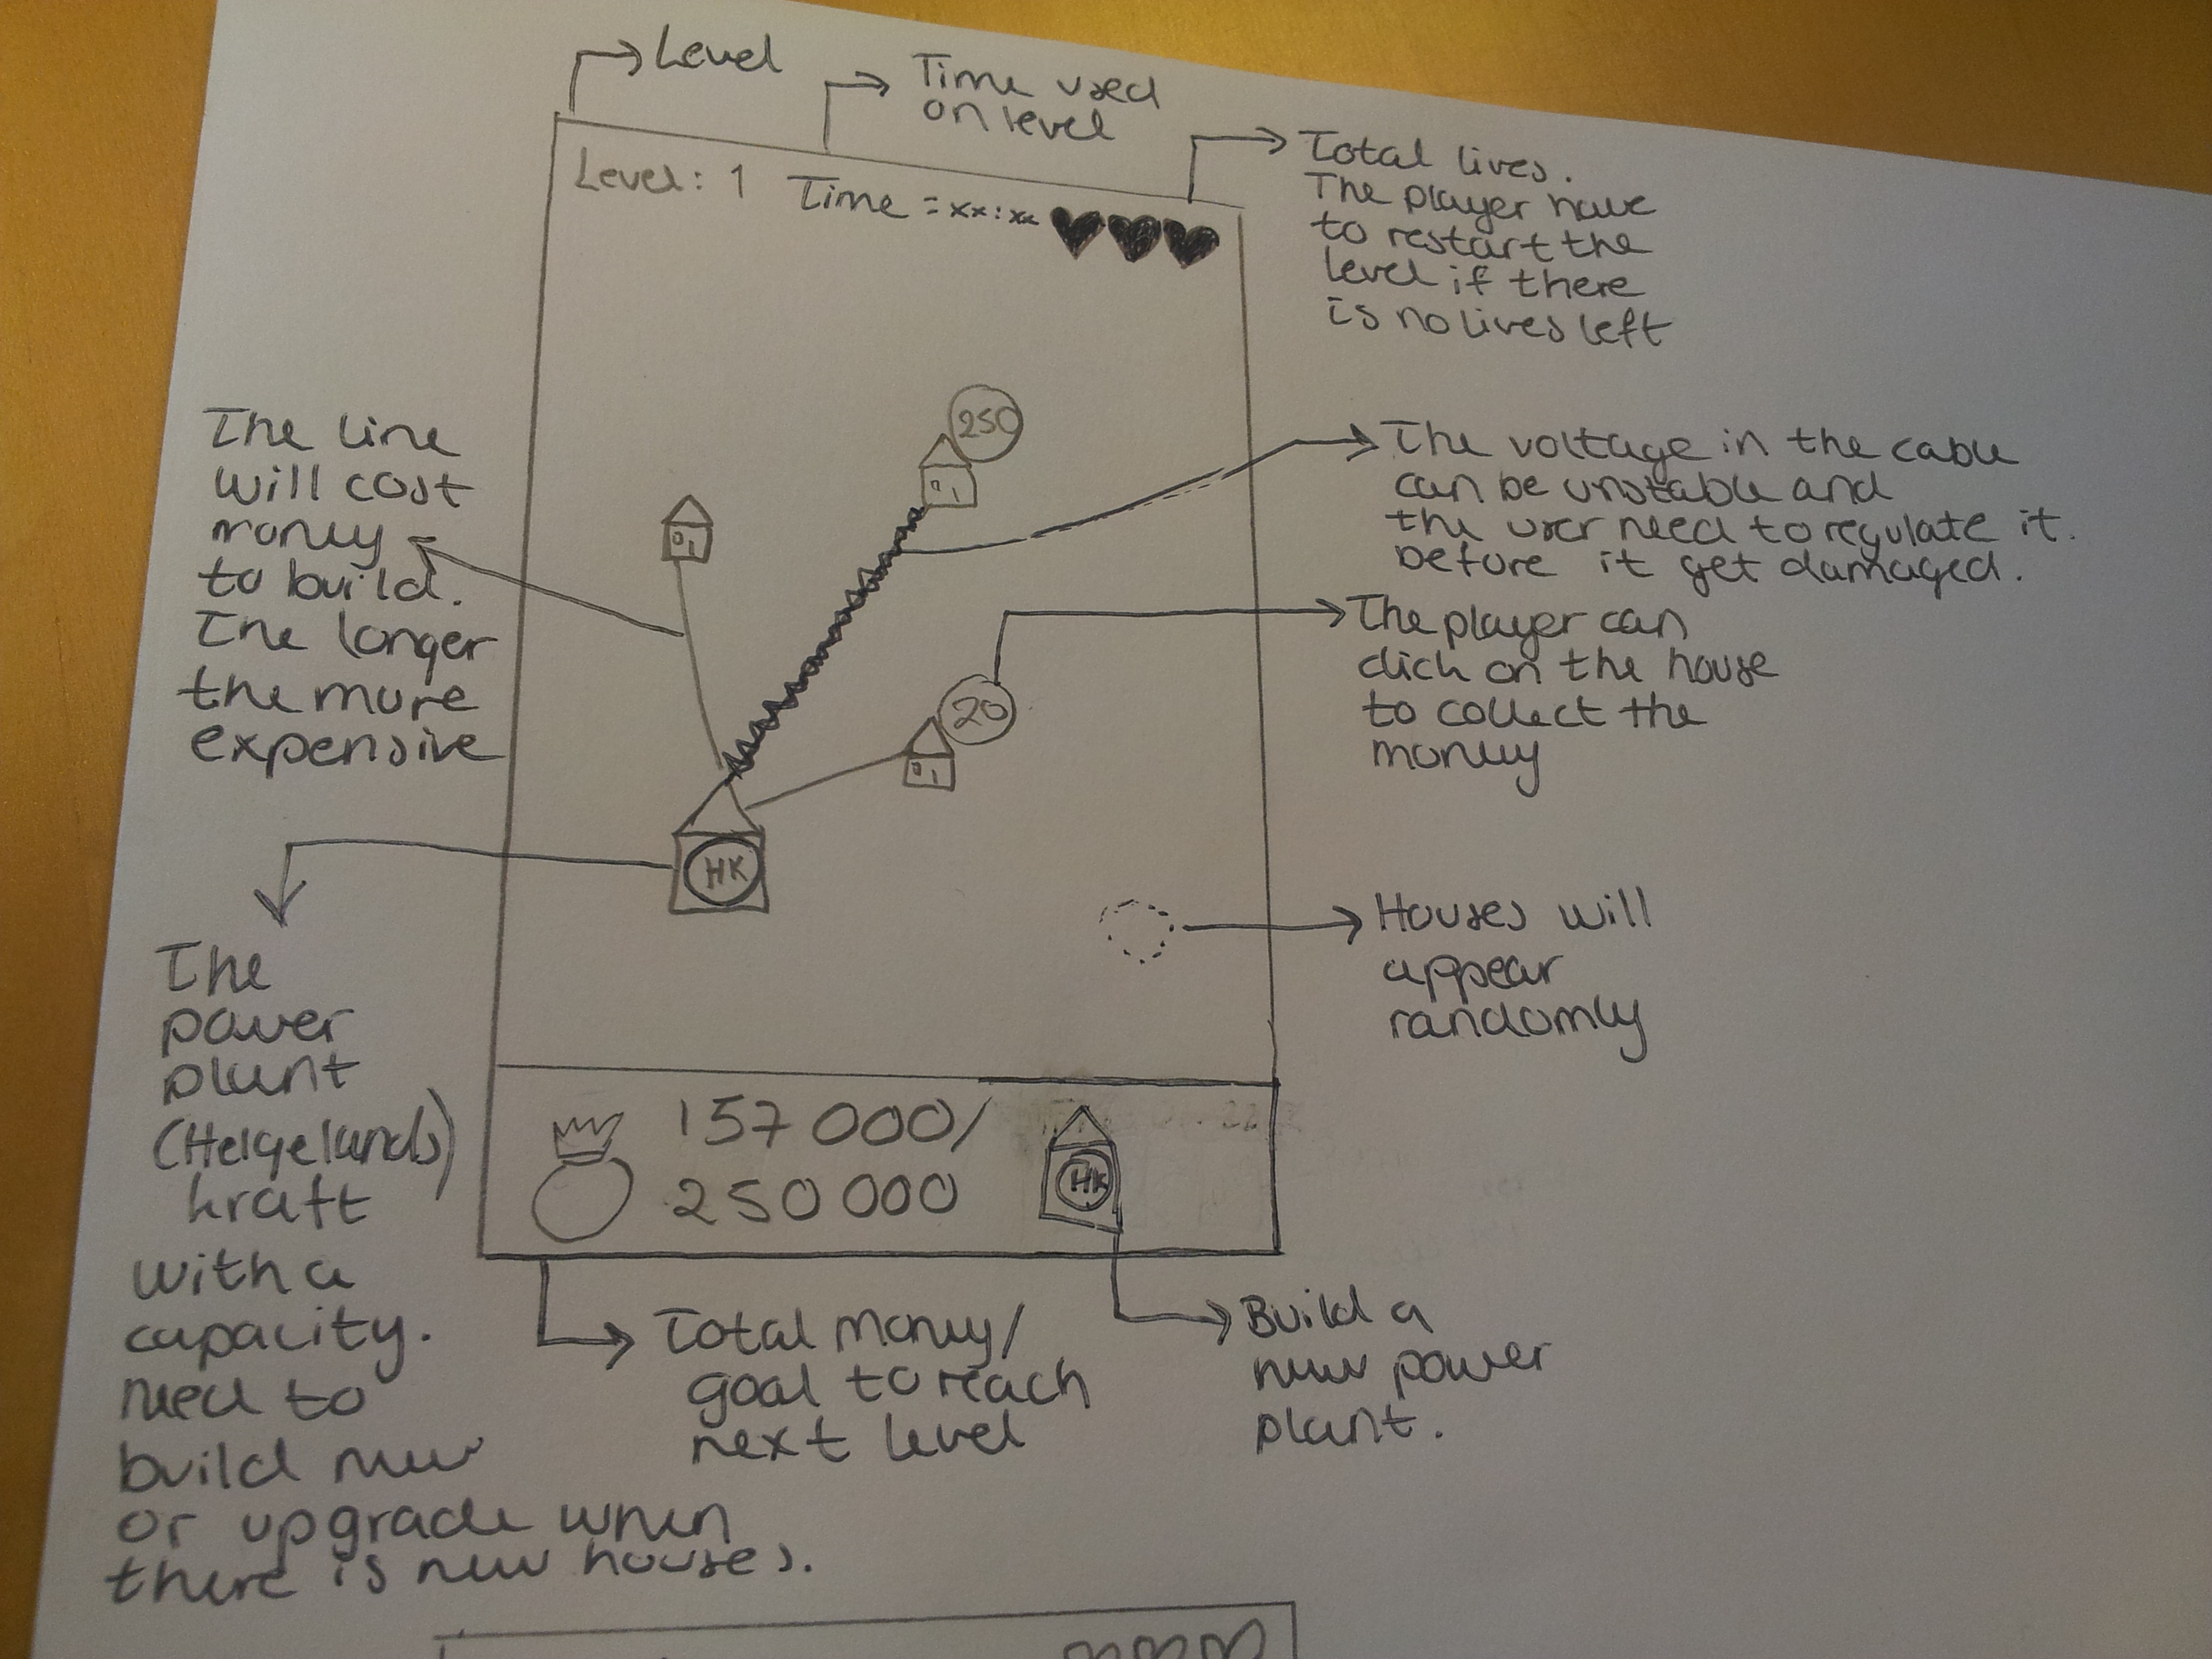
\includegraphics[scale=0.05]{pictures/gameConcept1}
		}
		\subfigure{
			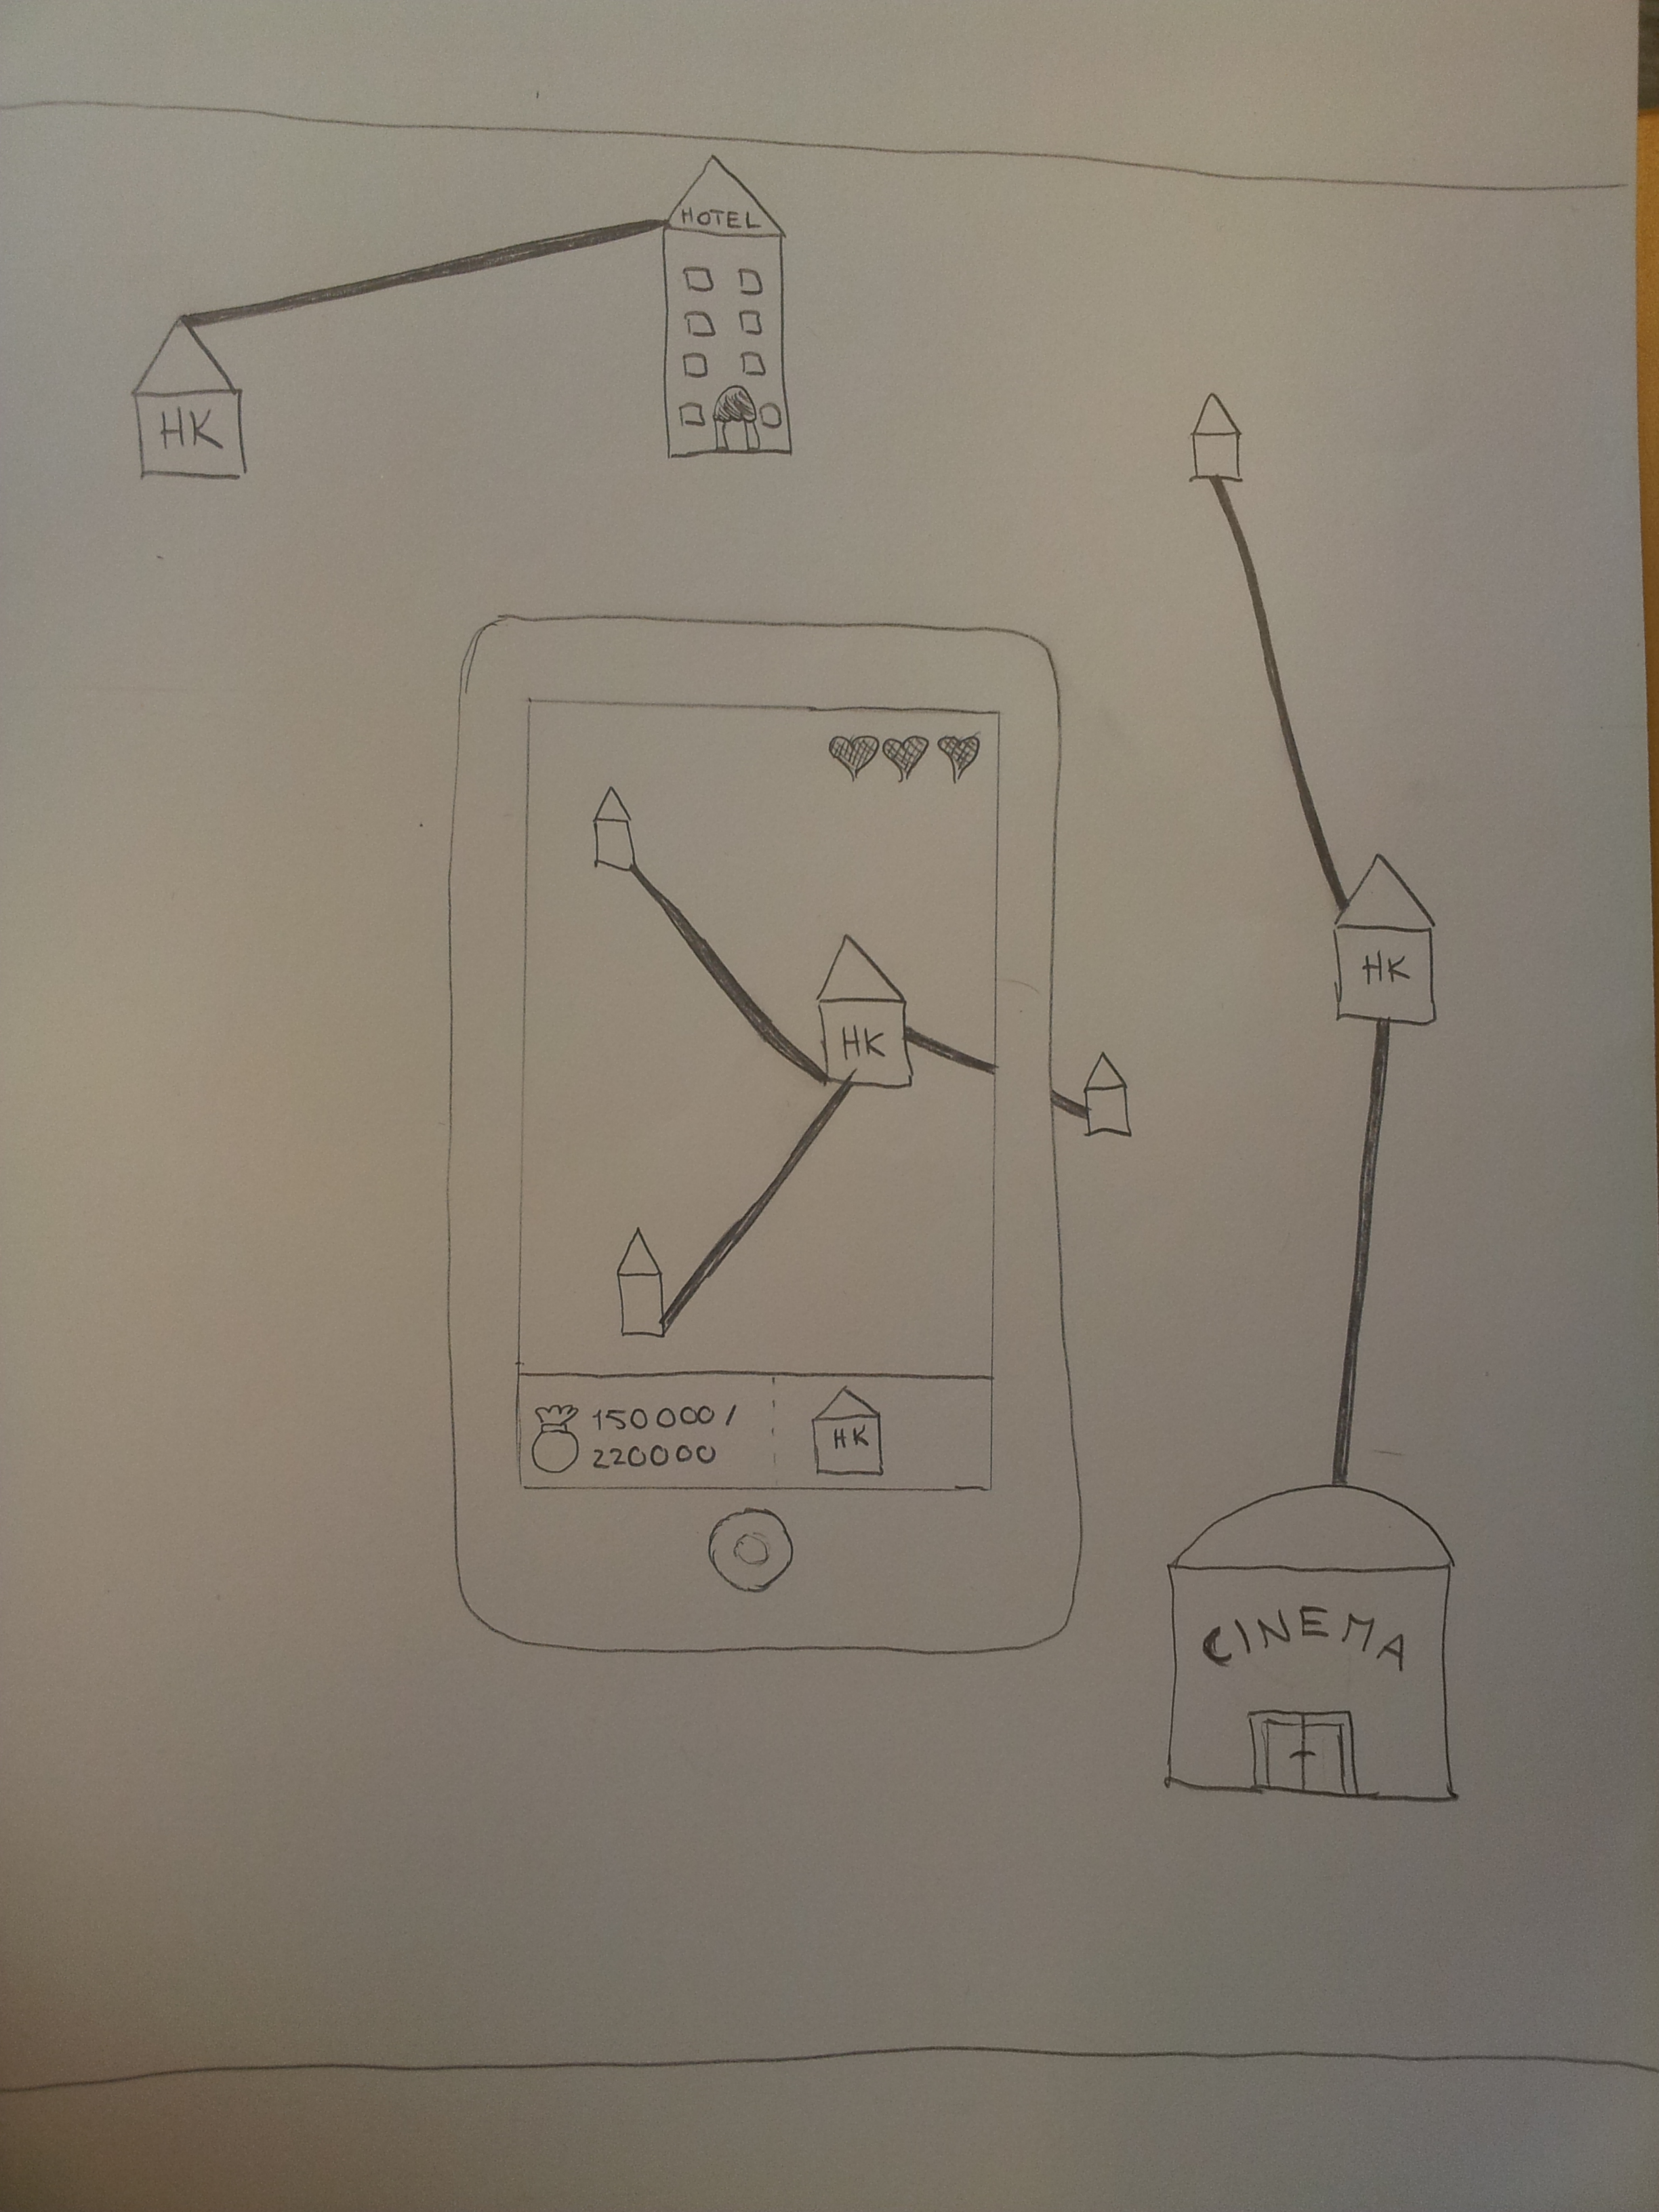
\includegraphics[scale=0.05]{pictures/gameConcept2}
		}
	\end{figure}



\subsection{Specification of the Requirements}

\subsection{Planning the first sprint}

\subsection{Group dynamics}

\subsection{Phase Results}
